\chapter{Arhitektura i dizajn sustava}
		
    Arhitektura sustava može se podijeliti na 3 podsustava:
    \begin{itemize}
        \item \textbf{web poslužitelj:} ključna komponenta Interneta. Njegove glavne zadaće uključuju raspoznavanje različitih URL-ova i procesuiranje HTTP zahtjeva čime se omogućuje komunikacija između klijenta i aplikacije. On pokreće web aplikaciju kojoj klijent pristupa pomoću web preglednika
        \item \textbf{web aplikacija:} program koji služi za ispunjenje klijentskih zahtjeva. Ovisno o zahtjevu, aplikacija upravlja dobivenim podacima (koje klijent šalje pomoću web preglednika), pristupa bazi podataka i vraća podatke pregledniku koji ih onda u odgovarajućem formatu prezentira klijentu
        \item \textbf{baza podataka:} služi za pohranu podataka koji se čuvaju tijekom rada te (u većini slučajeva) između različitih pristupa aplikaciji
    \end{itemize}
    
    %unos slike
		\begin{figure}[H]
			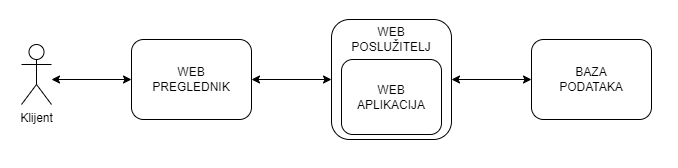
\includegraphics[scale=1]{slike/arhitektura.PNG} %veličina slike u odnosu na originalnu datoteku i pozicija slike
			\centering
			\caption{Arhitektura sustava}
			\label{fig:promjene}
		\end{figure}

	Programski jezici korišteni za razvoj aplikacije su Java zajedno sa Spring Boot radnim okvirom te JavaScript s radnim okvirom React. Arhitektura sustava temelji se na 4 sloja Spring Boot radnog okvira:
		
	\begin{itemize}
	    \item \textbf{presentation layer:} sastoji se od front-end dijela aplikacije te služi za rukovanje HTTP zahtjevima. Primljeni se zahtjevi ovjeravaju i prosljeđuju business sloju s kojim presentation sloj komunicira
	    \item \textbf{business layer:} ovaj sloj služi za rukovanje poslovnom logikom aplikacije. Sadrži klase za razne usluge te izvodi autentifikaciju i verifikaciju. Osim toga, služi kao posrednik presentation i persistence sloja
	    \item \textbf{persistence layer:} ovaj se sloj bavi logikom spremanja podataka - podatke koje dobiva od business sloja pretvara u upite nad bazom podataka te ih prosljeđuje database sloju i obrnuto
	    \item \textbf{database layer:} sloj koji izvodu CRUD (Create, Read, Update, Delete) operacije nad bazom podataka
	\end{itemize}
	

		\section{Baza podataka}
			
			%\textbf{\textit{dio 1. revizije}}\\
			
			Za potrebe sustava našeg projekta koristit ćemo relacijski bazu podataka. Osnovna građa baze je relacija. Relacija je tablica koja je definirana imenom i skupom atributa. Glavni zadatak baze podataka je brza i jednostavna pohrana, izmjena i dohvat podataka za daljnju obradu.
			Baza podataka ove aplikacije sastoji se od sljedećih tablica: 
			\begin{itemize}
				\item Korisnik
				\item Karta
				\item Borba
				\item Lokacija
				\item Vrsta lokacije
				\item Lokacija za potvrdu
			\end{itemize}
		
			\subsection{Opis tablica}
			

				%\textit{Svaku tablicu je potrebno opisati po zadanom predlošku. Lijevo se nalazi točno ime varijable u bazi podataka, u sredini se nalazi tip podataka, a desno se nalazi opis varijable. Svjetlozelenom bojom označite primarni ključ. Svjetlo plavom označite strani ključ}
				
				\textbf{Korisnik:} Ovaj entitet sadrži sve važne informacije o korisniku aplikacije. Sadrži atribute: korisničko ime, lozinka, fotografija, email, razina ovlasti, iban, fotografija osobne, bodovi i isključenje. Ovaj entitet u vezi je One-to-Many s entitetom Borba preko atributa korisničko ime korisnika, u vezi je One-to-Many s entitetom Karta preko atributa korisničko ime korisnika i u vezi je One-to-Many s entitetom Lokacija za potvrdu preko atributa korisničko ime korisnika.
				\begin{longtblr}[
					label=none,
					entry=none
					]{
						width = \textwidth,
						colspec={|X[6,l]|X[6, l]|X[20, l]|}, 
						rowhead = 1,
					} %definicija širine tablice, širine stupaca, poravnanje i broja redaka naslova tablice
					\hline \SetCell[c=1]{l}{\textbf{Korisnik}}	 \\ \hline[3pt]
					\SetCell{LightGreen}Korisničko ime & VARCHAR	&  	Jedinstveni identifikator korisnika  	\\ \hline
					Lozinka	& VARCHAR &   Hash lozinke	\\ \hline 
					Fotografija & LONGBLOB &  Fotografija korisnika \\ \hline 
					Email & VARCHAR	&  	Email korisnika	\\ \hline 
					Razina ovlasti	& VARCHAR &   Razina ovlasti korisnika \\ \hline 
					IBAN	& VARCHAR &   IBAN računa za uplatu za kartografa	\\ \hline 
					Fotografija osobne	& LONGBLOB &   Fotografija osobne iskaznice kartografa	\\ \hline 
					Bodovi	& INT &   Broj bodova koje je igrač osvojio	\\ \hline 
					Isključenje	& BOOLEAN &  Oznaka je li igrač trenutno isključen iz igre	\\ \hline 
				\end{longtblr}
				
				\textbf{Borba:} Ovaj entitet sadrži sve važne informacije vezane uz borbu. Sadrži atribute: id borba, korisničko ime protivnika, pobjednik, gubitnik i korisničko ime. Ovaj entitet u vezi je Many-to-One s entitetom Korisnik preko korisničkog imena.
				\begin{longtblr}[
					label=none,
					entry=none
					]{
						width = \textwidth,
						colspec={|X[6,l]|X[6, l]|X[20, l]|}, 
						rowhead = 1,
					} %definicija širine tablice, širine stupaca, poravnanje i broja redaka naslova tablice
					\hline \SetCell[c=1]{l}{\textbf{Borba}}	 \\ \hline[3pt]
					\SetCell{LightGreen}ID Borba & INT	&  	Jedinstveni identifikator borbe	\\ \hline
					Korisničko ime protivnika	& VARCHAR &   Korisničko ime protivnika u borbi	\\ \hline 
					Pobjednik	& VARCHAR &   Korisničko ime pobjednika u borbi	\\ \hline 
					Gubitnik	& VARCHAR &   Korisničko ime gubitnika u borbi	\\ \hline  
					\SetCell{LightBlue} Korisničko ime	& VARCHAR &   Korisničko ime korisnika koji je započeo borbu, (korisnik.korisnicko ime) 	\\ \hline 
				\end{longtblr}
			
				\textbf{Karta:} Ovaj entitet sadrži sve važne informacije vezane uz karte. Sadrži atribute: id karta, jačina karte, korisničko ime i id lokacija. Ovaj entitet u vezi je Many-to-One s entitetom Korisnik preko korisničkog imena i u vezi Many-to-one s entitetom Lokacija preko id lokacija.
				\begin{longtblr}[
					label=none,
					entry=none
					]{
						width = \textwidth,
						colspec={|X[6,l]|X[6, l]|X[20, l]|}, 
						rowhead = 1,
					} %definicija širine tablice, širine stupaca, poravnanje i broja redaka naslova tablice
					\hline \SetCell[c=1]{l}{\textbf{Karta}}	 \\ \hline[3pt]
					\SetCell{LightGreen}ID Karta & INT	&  	Jedinstveni identifikator karte	\\ \hline
					Jačina karte	& INT &   Jačina karte	\\ \hline 
					\SetCell{LightBlue} Korisničko Ime	& VARCHAR &   Jedinstveni identifikator korisnika kome pripada karta, (korisnik.korisnicko ime) 	\\ \hline
					\SetCell{LightBlue} ID Lokacija	& INT &   Jedinstveni identifikator lokacije, (lokacija.id lokacija)	\\ \hline 
				\end{longtblr}
			
				\textbf{Lokacija:} Ovaj entitet sadrži sve važne informacije vezane uz potvrđene lokacije. Sadrži atribute: id lokacije, naziv, opis, fotografija, jačina i id vrste lokacije. Ovaj entitet u vezi je Many-to-One s entitetom Vrsta lokacije preko id vrsta lokacije i One-to-Many s entitetom Karta preko id lokacija.
				\begin{longtblr}[
					label=none,
					entry=none
					]{
						width = \textwidth,
						colspec={|X[6,l]|X[6, l]|X[20, l]|}, 
						rowhead = 1,
					} %definicija širine tablice, širine stupaca, poravnanje i broja redaka naslova tablice
					\hline \SetCell[c=1]{l}{\textbf{Lokacija}}	 \\ \hline[3pt]
					\SetCell{LightGreen}ID Lokacije & INT	&  	Jedinstveni identifikator lokacije	\\ \hline
					Naziv	& VARCHAR &   Naziv lokacije	\\ \hline 
					Opis & VARCHAR &  Opis lokacije \\ \hline 
					Fotografija & LONGBLOB	&  	Fotografija lokacije	\\ \hline 
					Podatak za izračun jačine & VARCHAR	&  	Podatak za izračun početne jačine karte određene lokacije (grad-broj stanovnika,..)	\\ \hline 
					\SetCell{LightBlue} ID Vrste Lokacije	& INT &   Jedinstveni identifikator vrste lokacije (vrsta lokacije.id vrsta lokacije)	\\ \hline 
				\end{longtblr}
			
				\textbf{Vrsta lokacije:} Ovaj entitet sadrži sve važne informacije vezane uz vrste lokacija. Sadrži atribute: id vrsta lokacije i tip lokacije. Ovaj entitet u vezi je One-to-Many s entitetom Lokacija preko id vrsta lokacije i u vezi One-to-Many s entitetom Lokacija za potvrdu preko id lokacija za potvrdu.
				\begin{longtblr}[
					label=none,
					entry=none
					]{
						width = \textwidth,
						colspec={|X[6,l]|X[6, l]|X[20, l]|}, 
						rowhead = 1,
					} %definicija širine tablice, širine stupaca, poravnanje i broja redaka naslova tablice
					\hline \SetCell[c=1]{l}{\textbf{Vrsta Lokacije}}	 \\ \hline[3pt]
					\SetCell{LightGreen}ID Vrste Lokacije & INT	&  	Jedinstveni identifikator vrste lokacije  	\\ \hline
					Tip lokacije	& VARCHAR &   Naziv vrste lokacije	\\ \hline  
				\end{longtblr}
			
				\textbf{Lokacija za potvrdu:} Ovaj entitet sadrži sve važne informacije vezane uz lokacije za potvrdu. Sadrži atribute: id lokacije za potvrdu, naziv, opis, fotografija, jačina, korisničko ime kartografa, id vrste lokacije i korisničko ime. Ovaj entitet u vezi je Many-to-One s entitetom Vrsta lokacije preko id vrsta lokacije i Many-to-One s entitetom Korisnik preko korisničkog imena.
				\begin{longtblr}[
					label=none,
					entry=none
					]{
						width = \textwidth,
						colspec={|X[6,l]|X[6, l]|X[20, l]|}, 
						rowhead = 1,
					} %definicija širine tablice, širine stupaca, poravnanje i broja redaka naslova tablice
					\hline \SetCell[c=1]{l}{\textbf{Lokacija za potvrdu}}	 \\ \hline[3pt]
					\SetCell{LightGreen}ID Lokacije za potvrdu & INT	&  	Jedinstveni identifikator lokacije za potvrdu 	\\ \hline
					Naziv	& VARCHAR &   Naziv lokacije	\\ \hline 
					Opis & VARCHAR &  Opis lokacije \\ \hline 
					Fotografija & LONGBLOB	&  	Fotografija lokacije	\\ \hline 
					Podatak za izračun jačine & VARCHAR	&  	Podatak za izračun početne jačine karte određene lokacije (grad-broj stanovnika,..)	\\ \hline 
					Korisničko ime kartografa & VARCHAR &  Korisničko ime kartografa koji je će izvršiti potvrdu s terena \\ \hline 
					\SetCell{LightBlue} ID Vrste Lokacije	& INT &   Jedinstveni identifikator vrste lokacije (vrsta lokacije.id vrsta lokacije)	\\ \hline 
					\SetCell{LightBlue} Korisničko ime	& VARCHAR &   Jedinstveni identifikator korisnika koji je prijavio lokaciju za potvrdu (korisnik.korisničko ime)	\\ \hline 
				\end{longtblr}
				
				
			
			\subsection{Dijagram baze podataka}
				%\textit{ U ovom potpoglavlju potrebno je umetnuti dijagram baze podataka. Primarni i strani ključevi moraju biti označeni, a tablice povezane. Bazu podataka je potrebno normalizirati. Podsjetite se kolegija "Baze podataka".}
				
				 %unos slike
				\begin{figure}[H]
					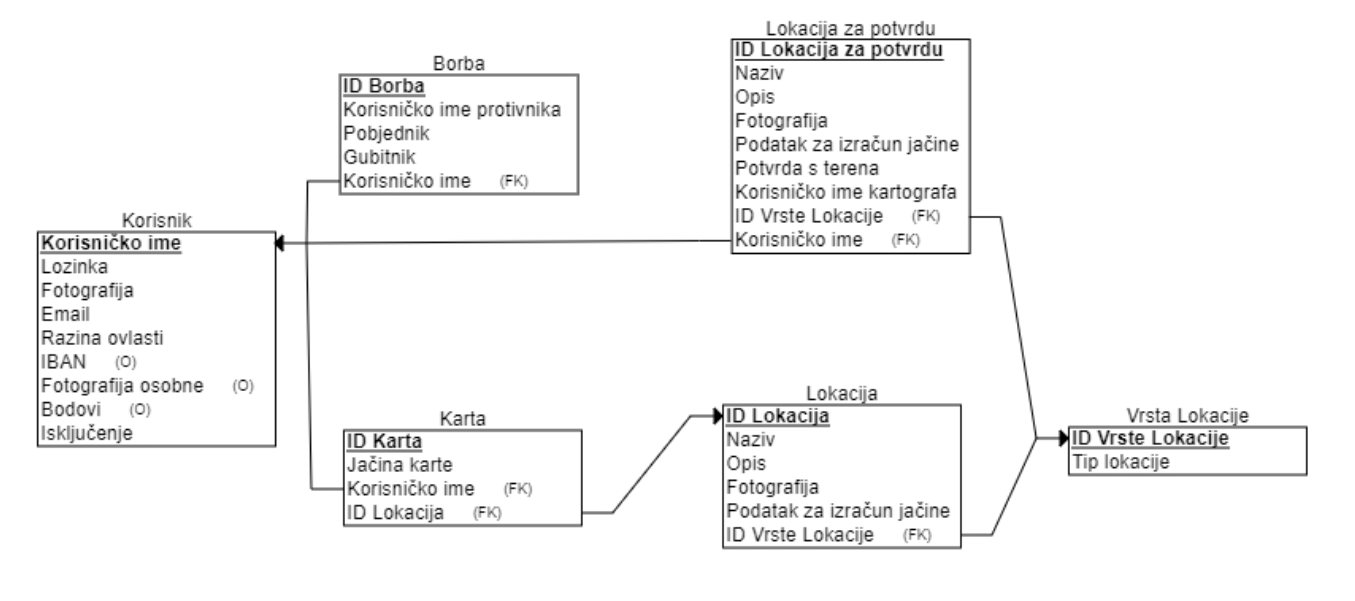
\includegraphics[width=\textwidth]{slike/Baza.PNG} %veličina slike u odnosu na originalnu datoteku i pozicija slike
					\centering
					\caption{Dijagram baze podataka}
					\label{fig:promjene}
				\end{figure}
			
			\eject
			
			
		\section{Dijagram razreda}
		
			%\textit{Potrebno je priložiti dijagram razreda s pripadajućim opisom. Zbog preglednosti je moguće dijagram razlomiti na više njih, ali moraju biti grupirani prema sličnim razinama apstrakcije i srodnim funkcionalnostima.}\\
			
			%\textbf{\textit{dio 1. revizije}}\\
			
			%\textit{Prilikom prve predaje projekta, potrebno je priložiti potpuno razrađen dijagram razreda vezan uz \textbf{generičku funkcionalnost} sustava. Ostale funkcionalnosti trebaju biti idejno razrađene u dijagramu sa sljedećim komponentama: nazivi razreda, nazivi metoda i vrste pristupa metodama (npr. javni, zaštićeni), nazivi atributa razreda, veze i odnosi između razreda.}\\

			Svaka od navedenih klasa predstavlja jednu od relacija baze podataka. Sve one nasljeđuju klasu Model. Na slici 4.4 prikazani su slojevi koji manipuliraju podacima vezanima uz korisnika - preko Controllera koji dohvaća unesene podatke preko Service klase koja ih prenosi do Repository klase koja podatke unosi u bazu i isti taj postupak obrnutim smjerom. Klase koje nasljeđuju RuntimeException koriste se kod implementacije logike upravljanja backend dijelom aplikacije te se bacaju kod raznih nedopuštenih ponašanja korisnika.
	
			 %unos slike
				\begin{figure}[H]
					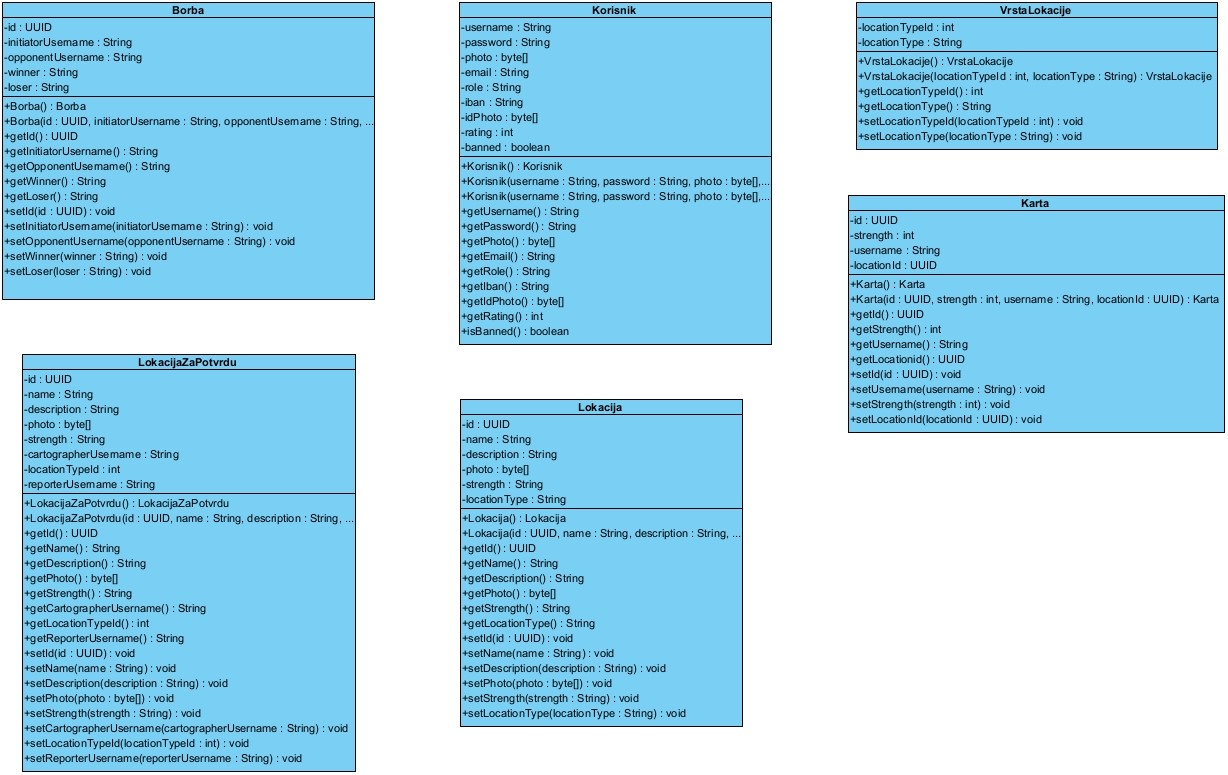
\includegraphics[width=\textwidth]{slike/model.jpg} %veličina slike u odnosu na originalnu datoteku i pozicija slike
					\centering
					\caption{Dijagram razreda - dio Model}
					\label{fig:promjene}
				\end{figure}
			\eject

			 %unos slike
				\begin{figure}[H]
					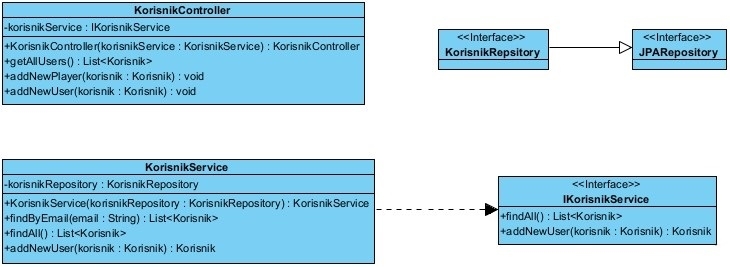
\includegraphics[width=\textwidth]{slike/service.jpg} %veličina slike u odnosu na originalnu datoteku i pozicija slike
					\centering
					\caption{Dijagram razreda - dio Service}
					\label{fig:promjene}
				\end{figure}

			 %unos slike
				\begin{figure}[H]
					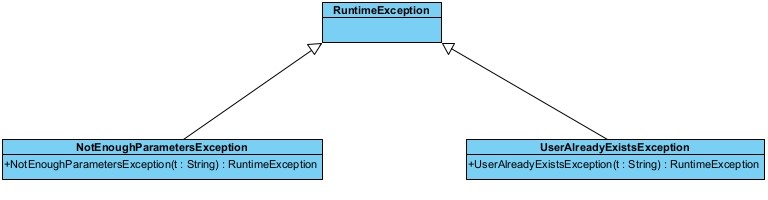
\includegraphics[width=\textwidth]{slike/exception.jpg} %veličina slike u odnosu na originalnu datoteku i pozicija slike
					\centering
					\caption{Dijagram razreda - dio Exceptions}
					\label{fig:promjene}
				\end{figure}

\iffalse
			
			\textbf{\textit{dio 2. revizije}}\\			
			
			\textit{Prilikom druge predaje projekta dijagram razreda i opisi moraju odgovarati stvarnom stanju implementacije}
			
			
			
			\eject
		
		\section{Dijagram stanja}
			
			
			\textbf{\textit{dio 2. revizije}}\\
			
			{Potrebno je priložiti dijagram stanja i opisati ga. Dovoljan je jedan dijagram stanja koji prikazuje \textbf{značajan dio funkcionalnosti} sustava. Na primjer, stanja korisničkog sučelja i tijek korištenja neke ključne funkcionalnosti jesu značajan dio sustava, a registracija i prijava nisu. }
			
			
			\eject 
		
		\section{Dijagram aktivnosti}
			
			\textbf{\textit{dio 2. revizije}}\\
			
			 \textit{Potrebno je priložiti dijagram aktivnosti s pripadajućim opisom. Dijagram aktivnosti treba prikazivati značajan dio sustava.}
			
			\eject
		\section{Dijagram komponenti}
		
			\textbf{\textit{dio 2. revizije}}\\
		
			 \textit{Potrebno je priložiti dijagram komponenti s pripadajućim opisom. Dijagram komponenti treba prikazivati strukturu cijele aplikacije.}
\fi